\chapter{Sensor-Embedded Teeth for Oral Activity Recognition}

The human mouth is one part of the human body that is almost always in constant use. We use our mouth to perform some of the most important daily functions, such as eating, drinking, speaking, coughing, breathing, and smoking. Because our mouth is an opening into assessing the health of the human body, it presents the opportunity for the placement of a strategic sensor for detecting human oral activities. For this study, we developed such an oral sensory system, where we explored the use of a small motion sensor embedded inside artificial teeth for the recognition of human oral activities. The detection of human oral activities can enable numerous health care applications, such as food and fluid intake monitoring.   
Previous research has explored wearable sensory devices installed in various locations of the upper body for detecting human oral activities. For example, Amft et al. [1] used an earphone-attached microphone sensor to record human chewing sounds and detect food types based on their acoustic profiles. Amft et al. [2] proposed another approach that combined surface Electromyography (EMG) and a microphone worn around the neck area to recognize low- or high-volume swallowing actions. BodyScope [3] placed an acoustic sensor around the neck area to recognize different oral activities (e.g., eating, drinking, speaking, laughing, and coughing) by analyzing sounds generated from the throat area. In comparison, our oral sensory system explores a unique sensor placement not on the human body, but inside the human body, specifically the mouth. Because a sensor placement inside the mouth has the advantage of being in proximity to where oral activities actually occur, this enables our oral sensory system to accurately capture the motion of oral activities. 
This paper presents the design and evaluation of this in-mouth oral sensory system, which uses a small accelerometer sensor embedded inside artificial teeth. Our motivation was based on our observation that most oral activities, such as chewing, drinking, speaking, and coughing, each produce a unique teeth motion. By recording and identifying teeth motion profiles for each oral activity, the proposed oral sensory system builds classifiers that distinguish different human oral activities. 

\begin{figure}[!ht]
\centering
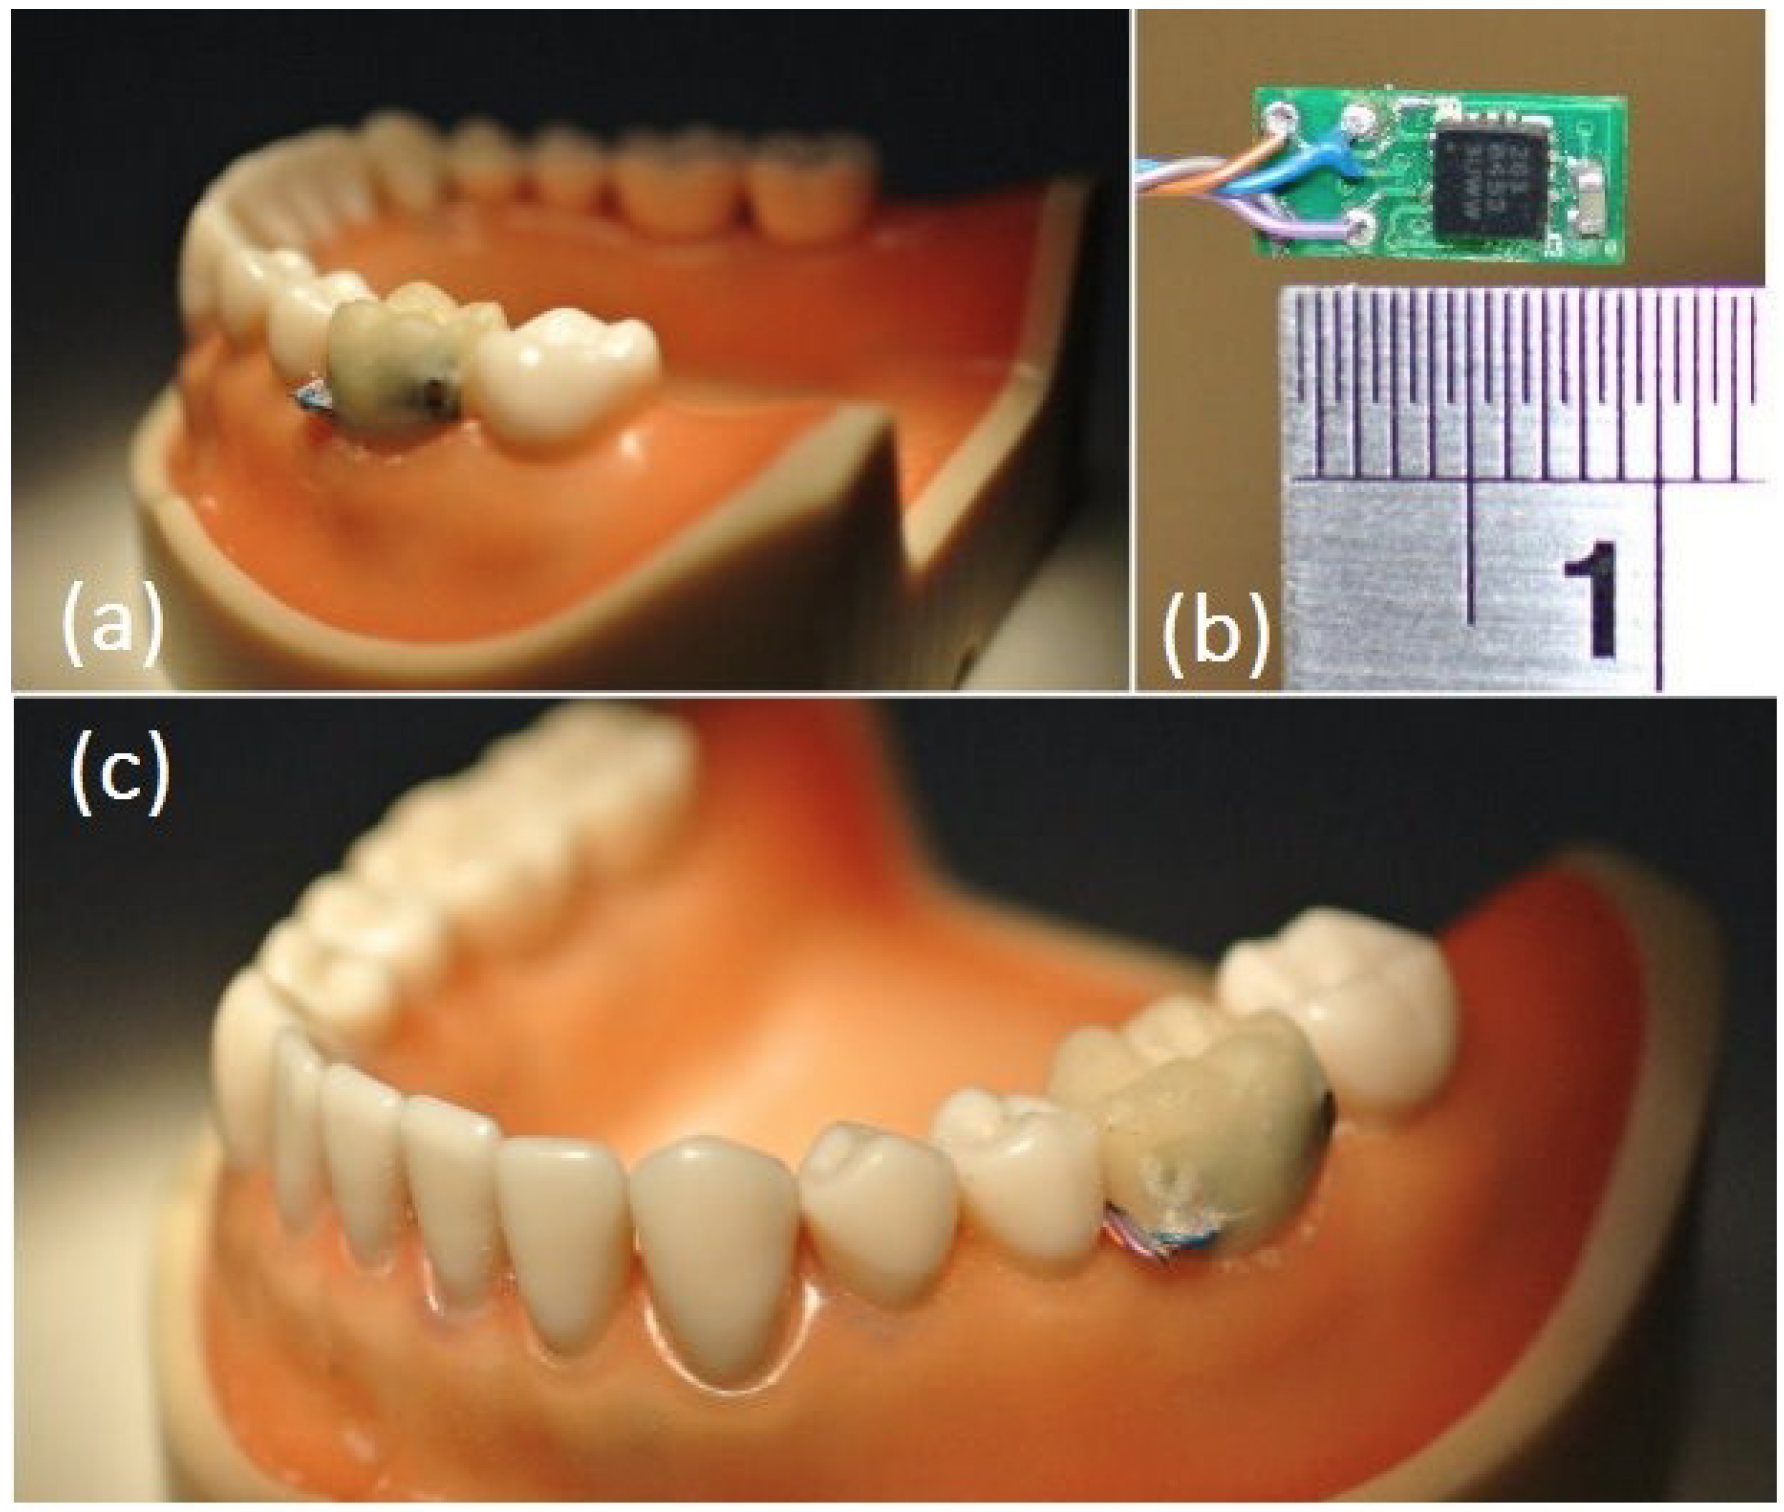
\includegraphics[width=14cm]{image/teeth}
\caption{The breakout board with (b) tri-axial accelerometer and (a)(c) sensor embedded denture.}
\label{teeth_overview}
\end{figure}

\section{System Overview}
The system consists of two main components: (a) an oral sensory unit; and (b) oral activity classifiers. 

\subsection{Oral Sensory Unit}
Figure 1(b) shows a small breakout board with a tri-axial accelerometer sized 4.5 mm x 10 mm. This small breakout board is sufficiently small to be embedded inside a removable artificial tooth, as shown in Figs. 1(a) and 1(c). To ensure that this sensor board is safe and saliva-proof for human mouth placement, we carefully coated the sensor board with dental resin. In actual system deployment, this sensor board would include a small Bluetooth radio capable of wirelessly transmitting sensor data to a nearby mobile phone for data analysis and oral activity recognition. In the current proof-of-concept system, we have yet to place a Bluetooth radio on this oral sensory unit; therefore, thin wires are used to connect the sensor board to an external data-logging device for data retrieval and power. These thin wires also protect users from accidentally swallowing the sensor units. 
Oral Activity Analysis
Oral activity recognition comprises the following three steps: (1) data preprocessing, (2) feature extraction, and (3) data classification. These steps are described as follows: 
\subsubsection{Data preprocessing}
The sampling rate of the accelerometer sensor is set to 100 Hz. The system first divides the accelerometer data into windows of 256 samples with a 50\% overlap between consecutive windows \cite{KristofVanLaerhoven:2000}. In each data window, the system extracts the time-domain and frequency-domain features shown in Table \ref{teeth_features}. 
Because people have different mouth and teeth specifications, sensor orientation can change for different users. Thus, accelerometer readings must be adjusted and calibrated using a rotation matrix. During the calibration phase, the proposed system asks users to hold their head straight and still for a few seconds during the application of Rodrigues' rotation formula to compute this rotation matrix. Each oral sensor unit has its own rotation matrix, which is used to transform its sensor readings from the device's coordinates to real-world coordinates. This normalization procedure reduces the negative effect of errors caused by varying device orientation. Because this normalization procedure reduces, but does not completely remove this error, the system also extracts orientation-independent features based on the magnitudes of x-, y-, and z-axis acceleration. For each sample at time t, its magnitude data is calculated as $\sqrt{x_{t}^{2}+y_{t}^{2}+z_{t}^{2}}$.


The normalized (orientation-dependent) feature set and the orientation-independent feature set have different characteristics. The normalized feature set retains separate information on tri-axial acceleration values, which are required for distinguishing activities involving both vertical and horizontal movements. In contrast, the orientation-independent feature set is based on the magnitude value, in which its precision is less affected by changes in device orientation; thus, it is suitable for distinguishing activities that depend on the movement scale.

\subsubsection{Feature extraction}
Table \ref{teeth_features} lists the time-domain and frequency-domain features extracted from each data window. Frequency-domain features are computed using the FFT algorithm. Both real and imaginary components of FFT coefficients in the 256-sample window are used to generate 256 features. Overall, the system trains activity classifiers by computing and extracting the following two feature sets: 807 features (269 features per axis acceleration) from the normalized feature set, and 269 features from the device-independent feature set.

\begin{table*}[!ht]
\centering
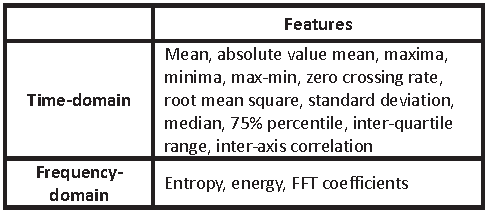
\includegraphics[width=14cm]{image/teeth_table1}
\caption{Adopted features for oral activity recognition.}
\label{teeth_features}
\end{table*}

\subsubsection{Training Classifiers}
Our system implements three classifiers: the C4.5 Decision Three (DT), the Multivariate Logistic Regression (MLR), and the Support Vector Machine (SVM). The SVM classifier uses the radial basis function kernel and one-against-one multiclass classification, and it is further optimized by an additional parameter selection and data scaling. To filter out redundant and irrelevant features, we performed feature selection based on the correlations between features. Low-relevance features with low correlation are filtered out. We adopted principal component analysis [5] as a feature selector, in which the number of relevant features was reduced to 137. 
For each classification algorithm of the DT, the MLR, and the SVM, we trained two classifiers: person-dependent and person-independent. A person-dependent classifier uses data from all users (i.e., 8 participants in our study) to train a generalized activity model for recognizing the oral activities of different users. Conversely, a person-independent classifier uses 7 users' data to train a specify activity model for recognizing remaining person's oral activities.

\section{Experimental Evaluation}
We conducted a laboratory experiment to evaluate the accuracies of different classification algorithms.

\subsection{Experimental Procedure}
Eight users (5 males and 3 females) participated in this experiment. They were asked to install the oral sensor unit inside their mouth while performing each of these four oral activities: chewing, drinking, talking, and coughing. Because it was not possible to customize a removable tooth for each participant, we used dental cement to fix the sensor units to each participant's tooth. For each activity, we collected 15 samples from each participant. Each sample consisted of 2.56 seconds of a specific activity performance. For the coughing data, participants were asked to cough continuously. For drinking data, participants were asked to drink a bottle of water. For chewing data, participants were asked to chew gum or to imitate the action. For speaking data, participants were asked to read a section of an article. We collected 480 activity samples from the 8 participants performing these four oral activities. Person-dependent and person-independent classifications used the same data set collected from the experiment.

\subsection{Results}
We conducted 10-fold cross-validation and leave-one-person-out cross-validation to measure the accuracies of the person-dependent and person-independent classifiers. For the person-dependent classifiers, each round of cross-validation involved using all of each participant's data for both training and testing. Table \ref{teeth_pdc} shows the mean F-measure accuracy results. The SVM (93.8\%) classifier outperforms both the DT (52.2\%) and MLR (60.5\%) classifiers.  

For the person-independent classifiers, each round of cross-validation involved using 7 participants' data for training, and the remaining participant's data for testing. Table \ref{teeth_pdc} shows the mean F-measure accuracy results. Again, the SVM (59.8\%) classifier outperformed both the DT (40.8\%) and MLR (55.9\%) classifiers. Reasons for the low-accuracy result in the person-independent classifier are as follows.
First, because people's teeth and mouth structure are different, their sensor placements are also (slightly) different, thus creating variations in the motion data. Second, people perform oral activities differently; for instance, some people chew or talk faster, slower, harder, or softer. It is possible to improve the accuracy of person-independent classification by extending the training set to include different sensor placements and oral activity types.
\newpage

\begin{table*}[!ht]
\centering
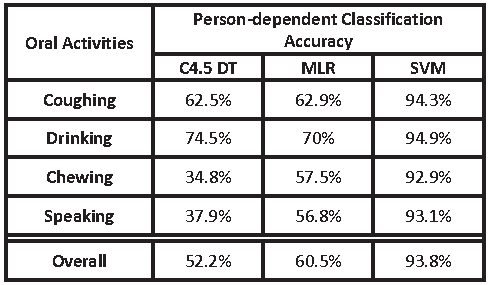
\includegraphics[width=14cm]{image/teeth_table2}
\caption{F-measure accuracy of oral activity recognition with a person-dependent classifier.}
\label{teeth_pdc}
\end{table*}

\begin{table*}[!ht]
\centering
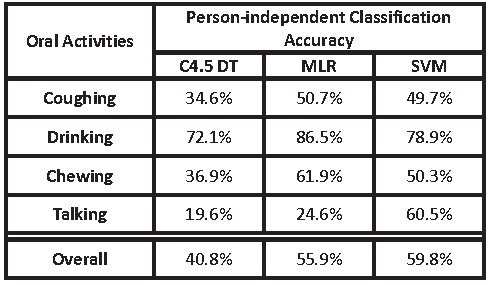
\includegraphics[width=14cm]{image/teeth_table3}
\caption{F-measure accuracy of oral activity recognition with a person-independent classifier.}
\label{teeth_pidc}
\end{table*}

\newpage
\section{Discussion}
This is a feasibility study of an oral sensory system that detects human oral activities. We identified the following challenges for the proposed oral sensory system.

\subsubsection{Data logging and transmission}
If an application does not require real-time monitoring, sensory data can be temporarily stored on the sensor device. When users remove their artificial teeth, for example, for disinfection and storage, small electrodes on the surface of the artificial teeth are used to connect to the sensor board and retrieve stored sensor data. For a real-time monitoring application, the sensor board must have a low-power wireless radio (e.g., Bluetooth) to transmit sensor data to a nearby smartphone for data analysis and activity recognition. Another possible data transmission medium is intra-body communication \cite{Hachisuka:2003}, which has lower power consumption compared to wireless radio communication.

\subsubsection{Energy}
Because users must remove artificial teeth for daily disinfection and storage, we surmise that a recharging and storage station will be required, similar to that of an electric toothbrush, in which users would place the cleaned artificial teeth on this station for battery recharging and data retrieval. 

\subsubsection{Safety}
Because of the sensor placement inside the mouth, the safety concern is paramount. All electronic components must be sealed securely and tightly. In the event that the sensor units are mistakenly swallowed, they will pass the human body without causing any harm. Its safety requirements are similar to those of capsule endoscopy, in which patients swallow a camera pill. Because our current prototype (Figure \ref{teeth_overview}) was not considered safe, we attached a safety string to the sensor unit so that participants would not be able to swallow it.

\subsection{Summary}
For this study, we designed and developed an oral sensory system that can recognize human oral activities. Our results from a laboratory experiment with 8 participants demonstrate the feasibility of this oral sensory system in recognizing the following four human oral activities: speaking, chewing, drinking, and coughing. We found that a person-dependent SVM classifier achieved a high F-measure accuracy of 93.8$\%$, whereas a person-independent SVM classifier achieved only an F-measure accuracy of 59.8$\%$. 
Because the mouth is an opening into human health, this oral sensory system has the potential to enhance exiting oral-related healthcare monitoring applications such as dietary tracking. 

\let\cleardoublepage\clearpage
